
\documentclass[ms.tex]{subfiles}

\begin{document}

\section{Predicted Specific SN Ia Rates}
\label{sec:predictions}

\begin{figure*}
\centering
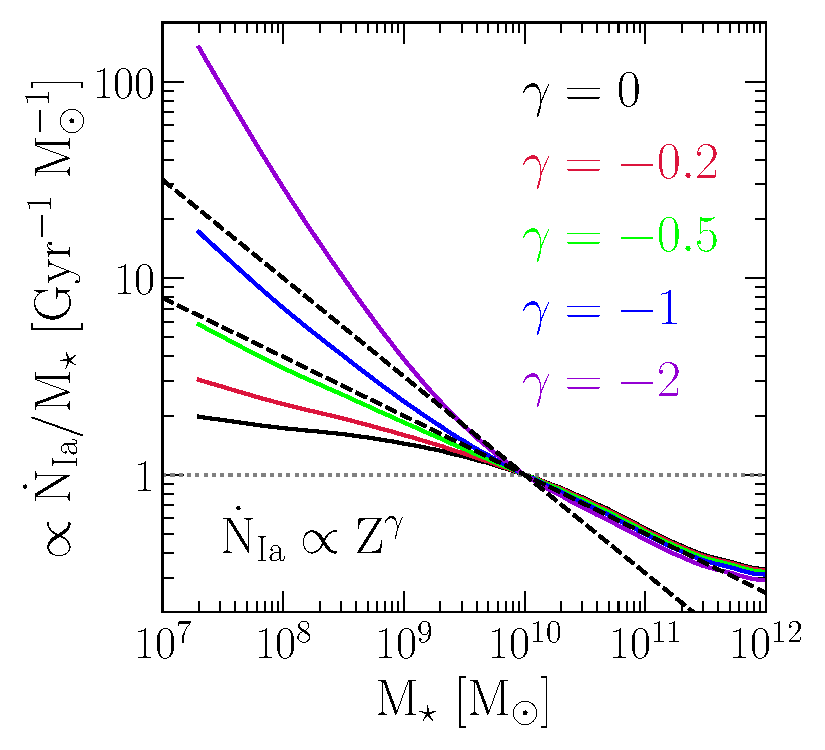
\includegraphics[scale = 0.55]{umachine_iarate_metdep.pdf}
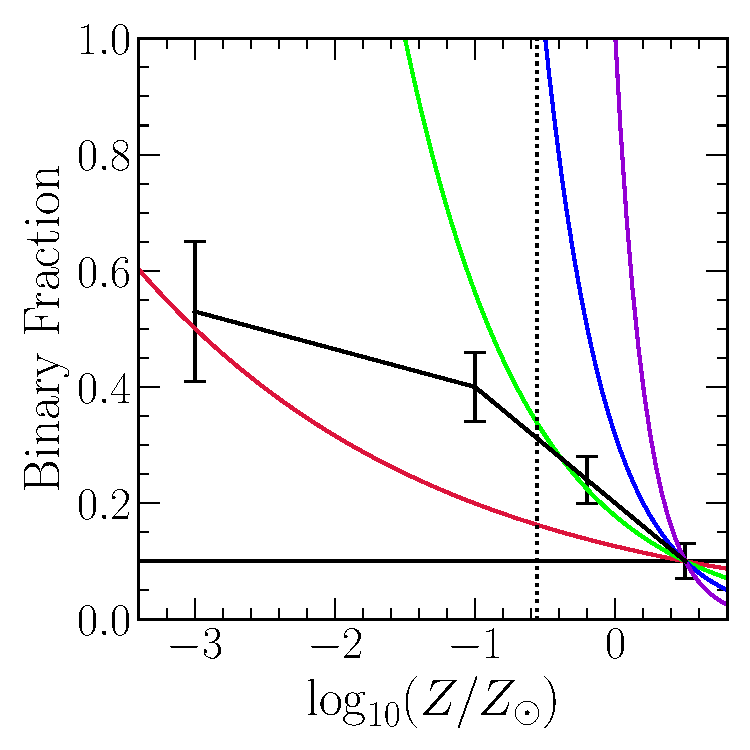
\includegraphics[scale = 0.55]{binaries_zscaling.pdf}
\caption{
\textbf{Left}: Theoretically predicted scalings of the specific SN Ia rate with
various assumptions about the metallicity dependence of the rate.
\textbf{Right}: Various metallicity scalings in comparison with the
close-binary fraction observed in APOGEE~\citep{Moe2019}.
}
\label{fig:specia_metdep}
\end{figure*}

\begin{itemize}

	\item In this section we combine the variations in SFHs and metallicities
	across the~$10^7 - 10^{12}~\msun$ range as discussed
	in~\S~\ref{sec:galprops}.
	Given the present-day stellar mass of a galaxy, we compute its SFH as a
	function of lookback time by interpolating between the stellar masses and
	snapshot times included in the~\um~predictions.\footnote{
		\url{https://www.peterbehroozi.com/data.html}. We interpolate linearly
		in both stellar mass and lookback time and not in the log of either
		quantity.
	}
	We then compute the specific SN Ia rate according to equation
	\refp{eq:specia} given the implied SFH and a~$\tau^{-1}$ DTD.
	We artificially amplify the implied rate by a factor of~$Z^{\gamma}$
	where the power-law index~$\gamma$ is a free parameter and~$Z$ is the metal
	abundance by mass implied by the~\citet{Zahid2014} MZR computed via
	$Z = Z_\odot 10^\text{[O/H]}$.
	Here we take~$Z_\odot = 0.014$ according to~\citet{Asplund2009}, but this
	choice has no impact as we normalize all of our specific SN Ia rates to 1
	at~$10^{10}~\msun$ following~\citet{Brown2019} and~\citet{Gandhi2022}.

	\item We show the results of this procedure in the left panel of Fig.
	\ref{fig:specia_metdep} for~$\gamma = 0, -0.2, -0.5, -1$ and~$-2$ in
	comparison to the~$\dot{N}_\text{Ia} / M_\star \sim M_\star^{-0.5}$ and
	$\dot{N}_\text{Ia} / M_\star \sim M_\star^{-0.3}$ scalings found by
	\citet{Brown2019} and~\citet{Gandhi2022}, respectively.
	The metallicity dependence has a significant impact only below
	$\sim10^9~\msun$, a result which arises due to the shape of the MZR: this
	is the mass above which the MZR flattens considerably.
	Assuming no metallicity dependence (i.e.~$\gamma = 0$), these calculations
	suggest that the variations in SFHs between~$\sim10^7$ and~$10^{10}~\msun$
	can only produce a factor of~$\sim$2 increase in the specific SN Ia rate
	at low stellar masses.
	Within the observational and theoretical uncertainties, the~$\gamma = -0.5$
	case is generally consistent with a mass dependence of~$M_\star^{-0.3}$.
	\citet{Gandhi2022} advocate for a similar scaling with~$Z$, additionally
	demonstrating that incorporating this metallicity dependence into the
	FIRE-2\footnote{
		Feedback In Realistic Environments,~\url{https://fire.northwestern.edu/}
	}
	cosmological zoom-in simulations~\citep{Hopkins2018} leads to better
	agreement with the stellar masses and iron abundances measured by
	\citet{Gallazzi2005} and~\citet{Kirby2013}.
	The scaling of~$M_\star^{-0.5}$ as found by~\citet{Brown2019}, however,
	would require a yet stronger scaling of~$\gamma \approx -1.5$.

	\item In the right panel of Fig.~\ref{fig:specia_metdep}, we compare these
	same scalings with~$Z$ to the close binary fractions measured by
	\citet{Moe2019}.
	We mark the position of~$Z \approx 10^{-0.6} Z_\odot$, the characteristic
	metallicity of a~$10^{7.2}~\msun$ galaxy according to~\citet{Zahid2014}.
	Within the range of metallicities implied by the stellar masses that we
	consider in the present paper, the dependence of the close binary fraction
	on metallicity is broadly consistent with~$Z^{-0.5}$.
	If the~$M_\star^{-0.3}$ scaling found by~\citet{Gandhi2022} is accurate,
	then this suggests that the increase of the specific SN Ia rate with
	decreasing stellar mass can be explained in its entirety by the combination
	of the how SFHs depend on stellar mass and a higher close binary fraction
	due to the lower metallicities in dwarf galaxies.
	If one instead takes~$Z \approx 0.1 Z_\odot$ for a~$\sim10^{7.2}~\msun$
	as suggested by the~\citet{Andrews2013} MZR, then there is a slight
	tension between a~$Z^{-0.5}$ scaling and the close binary fraction measured
	by~\citet{Moe2019}.
	If a~$Z^{-0.5}$ scaling is accurate, then in this case it would be
	reasonable to suggest that any additional SNe Ia that the increase in the
	close binary fraction could not produce are supplied by lower metallicity
	stars leaving behind higher mass WDs as postulated by~\citet{Kistler2013},
	though even in this case, the scaling of the close binary fraction with
	metallicity can explain the majority of the effect.

	\item These are indeed highly simplified calculations in several regards.
	First, we assume the characteristic SFH predicted by a SAM at all stellar
	masses.
	This is reasonble for computing expected mean trends, but in principle, the
	underlying galaxy population should occupy a distribution of rates at
	fixed stellar mass due to variations in their SFHs.
	Second, we have assumed that all galaxies lie perfectly on the MZR.
	This should also be sufficient for computing mean trends, but similarly,
	galaxies should populate a distribution of metallicities at fixed stellar
	mass.
	Third, our metallicity scaling of~$Z^{\gamma}$ where
	$Z = Z_\odot 10^\text{[O/H]}$ assumes that all SNe Ia in any galaxy arise
	from stellar populations at exactly the gas-phase abundance implied by the
	MZR.
	This is nonetheless a reasonable assumption because models of galactic
	chemical evolution incorporating an exchange of baryons with the
	surrounding medium via inflows and outflows suggest that galaxies should
	rapidly approach an equilibrium abundance in which the production of
	new metals is balanced by losses to star formation and outflows
	\citep{Larson1972, Weinberg2017}.
	This would imply that the young stellar populations which dominate the SN
	Ia rate (see Fig.~\ref{fig:sfhs} and discussion in~\S~\ref{sec:galprops})
	should be of similar metallicities -- at least on average.
	Although the close binary fraction is known to increase at low abundances
	in APOGEE~\citep{Badenes2018, Moe2019},~\citet{Mazzola2020} find that the
	binary fraction decreases for stars with high [$\alpha$/Fe] ratios at
	fixed [Fe/H], suggesting that the detailed chemical composition may
	significantly impact stellar multiplicity.
	Furthermore, the abundances of metals in stars is a many-dimensional
	quantity~\citep[e.g.][]{Ting2022}.
	However, a theoretical understanding of the metallicity dependence of SN Ia
	rates is a relatively new topic in the literature.
	A first-order understanding of how the rates scale with the absolute metal
	abundance in statistically average galaxies must be attained before
	considering how it should scale with the detailed chemical composition of
	the progenitor populations.



	% To this end, we compute the SFH~$\dot{M}_\star$ of a galaxy as a function
	% of its present-day stellar mass and lookback time by interpolating between the
	% stellar masses and snapshot times included in the~\um~predictions.\footnote{
	% 	\url{https://www.peterbehroozi.com/data.html}
	% }
	% To explore scalings of the SN Ia rate with metallicity of various
	% strengths, we artificially amplify

\end{itemize}

\end{document}
